% =====================================================================
% Apresentação do trabalho final (Entrega 2) - Instrumentação Eletrônica
% Baseado no backup slide das reuniões do Projeto Radar.
% Compilar: pdflatex apresentacao.tex (duas vezes)
% =====================================================================
\documentclass[aspectratio=169]{beamer}
\usepackage[utf8]{inputenc}
\usepackage[T1]{fontenc}
\usepackage[brazil]{babel}
\usepackage{lmodern}
\usepackage{graphicx}
\usepackage{booktabs}
\usepackage{tikz}
\graphicspath{{figuras/}}

\setbeamertemplate{navigation symbols}{}
\setbeamertemplate{footline}[frame number]
\setbeamertemplate{itemize items}[circle]
\setbeamertemplate{blocks}[rounded]
\setbeamercolor{block title}{bg=blue!15,fg=blue!50!black}
\setbeamercolor{block body}{bg=blue!4}

% texto à esquerda, gráfico à direita
% uso: \slidegrafico{texto}{arquivo da figura}{nome do código}
\newcommand{\slidegrafico}[3]{%
  \begin{columns}[T]
  \begin{column}{0.43\textwidth}
  \small
  #1
  \end{column}
  \begin{column}{0.57\textwidth}
  \vspace{0.4cm}
  \includegraphics[width=\textwidth]{#2}\\[2pt]
  \centering\scriptsize Código: \texttt{\detokenize{#3}}
  \end{column}
  \end{columns}}

\title{Calibração e medição do ângulo de inclinação\\com o acelerômetro do MPU 6050}
\subtitle{Instrumentação Eletrônica para Engenharia -- Trabalho final}
\author{Felipe de Castro Quixabeira \and Gabriel Celestino de Almeida}
\institute{UnB -- FCTE}
\date{24/11/2026}

\begin{document}

\begin{frame}
\titlepage
\end{frame}

% ---------------------------------------------------------------------
\begin{frame}{Objetivo}
\begin{columns}[T]
\begin{column}{0.5\textwidth}
\small
\begin{itemize}
\item Calibrar o acelerômetro do MPU 6050: ganho e offset de cada eixo
\item Medir o ângulo de inclinação de um mecanismo com um grau de liberdade
\item Comparar com um transferidor e levantar o erro ao longo da faixa
\end{itemize}
\vspace{6pt}
\textbf{Montagem}
\begin{itemize}
\item ESP32 lendo o MPU 6050 pelo I$^2$C
\item Dados pela serial para o computador
\end{itemize}
\end{column}
\begin{column}{0.45\textwidth}
\centering
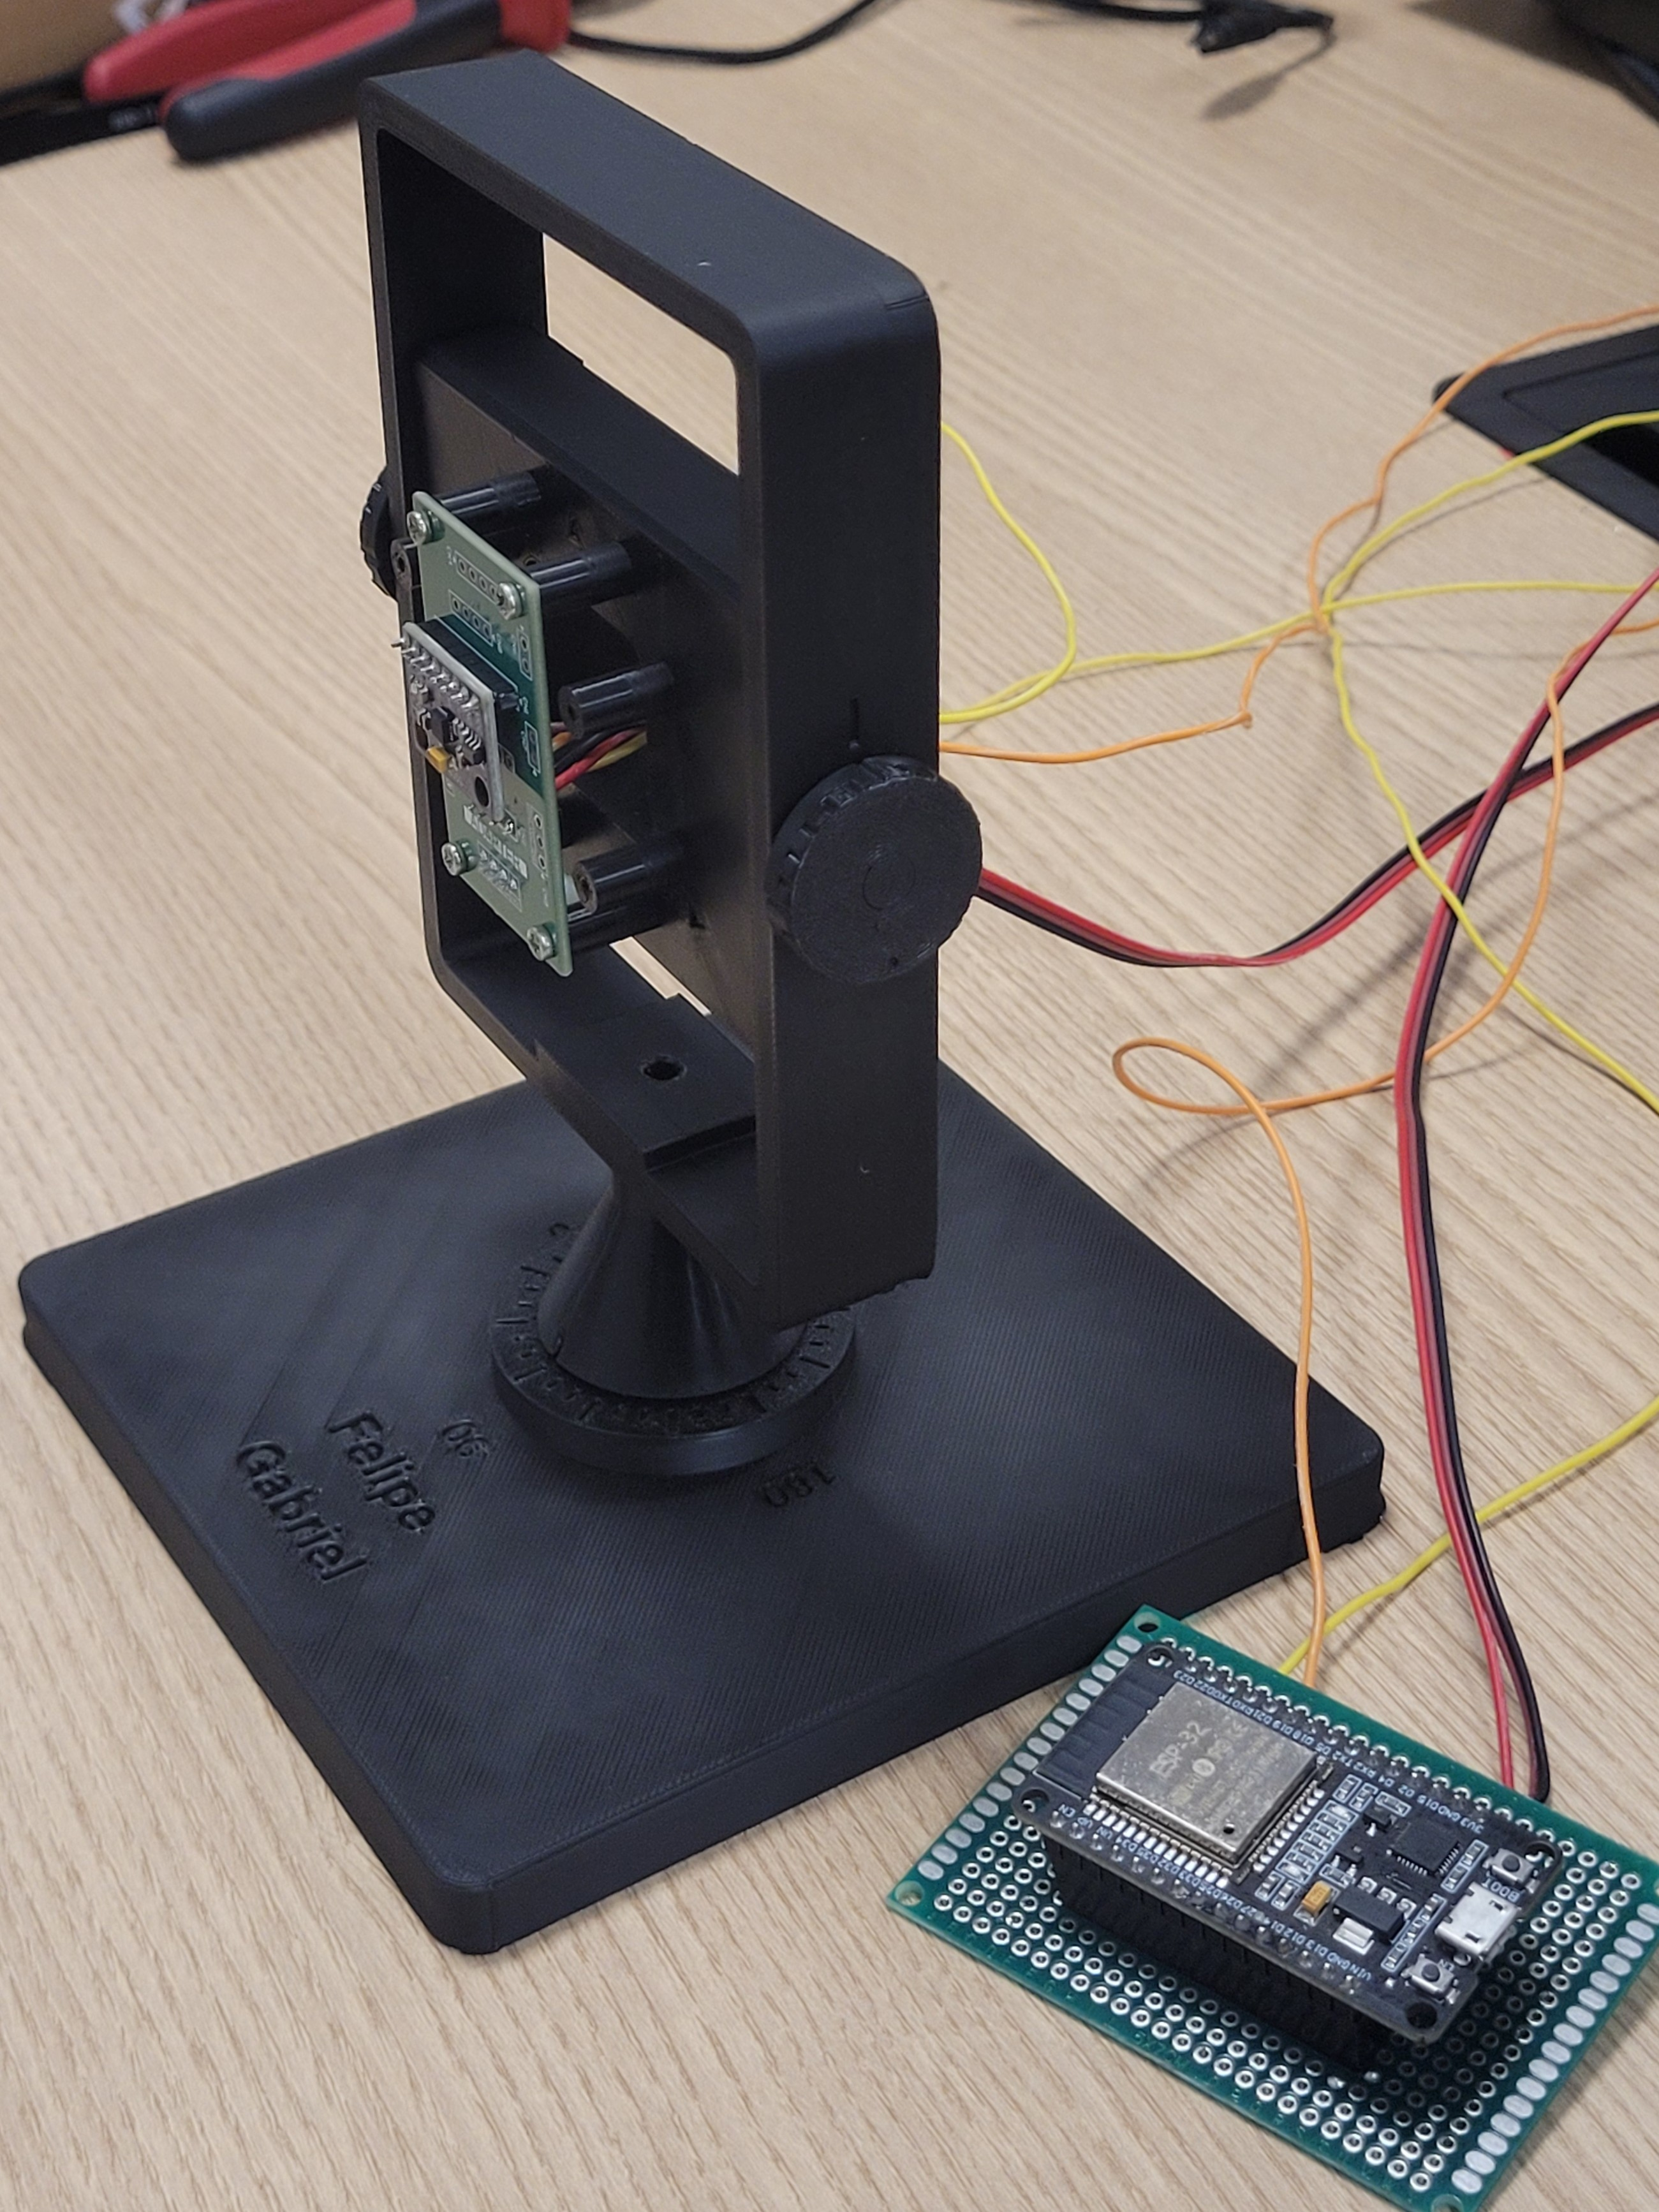
\includegraphics[height=6cm]{base__isometrico.jpg}\\[2pt]
\scriptsize Base montada com o sensor
\end{column}
\end{columns}
\end{frame}

% ---------------------------------------------------------------------
\begin{frame}{Ligação do ESP32 com o MPU 6050}
\begin{columns}[T]
\begin{column}{0.3\textwidth}
\small
\begin{tabular}{@{}ll@{}}
\toprule
MPU 6050 & ESP32 \\
\midrule
VCC & 3V3 \\
GND & GND \\
SDA & GPIO21 \\
SCL & GPIO22 \\
AD0 & GND \\
\bottomrule
\end{tabular}

\vspace{8pt}
\begin{itemize}
\item AD0 no GND: endereço \texttt{0x68}
\item Alimentação em 3,3\,V
\end{itemize}
\end{column}
\begin{column}{0.68\textwidth}
\vspace{0.3cm}
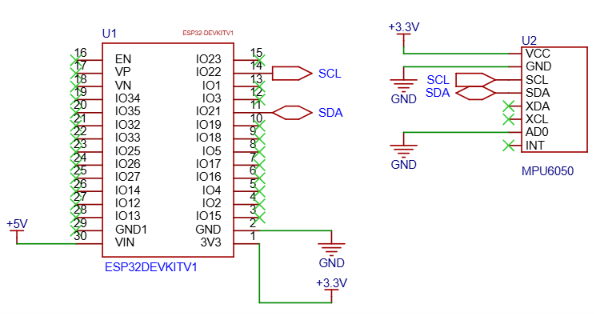
\includegraphics[width=\textwidth]{esquematico.png}
\end{column}
\end{columns}
\end{frame}

% ---------------------------------------------------------------------
\begin{frame}{Mecanismo de validação}
\begin{columns}[T]
\begin{column}{0.36\textwidth}
\small
\begin{itemize}
\item Base impressa em 3D
\item O sensor fica preso num berço que gira em torno de um eixo horizontal
\item Um dos eixos trava o berço no ângulo do ensaio
\item Referência: transferidor com resolução de $1^\circ$
\end{itemize}
\end{column}
\begin{column}{0.62\textwidth}
\centering
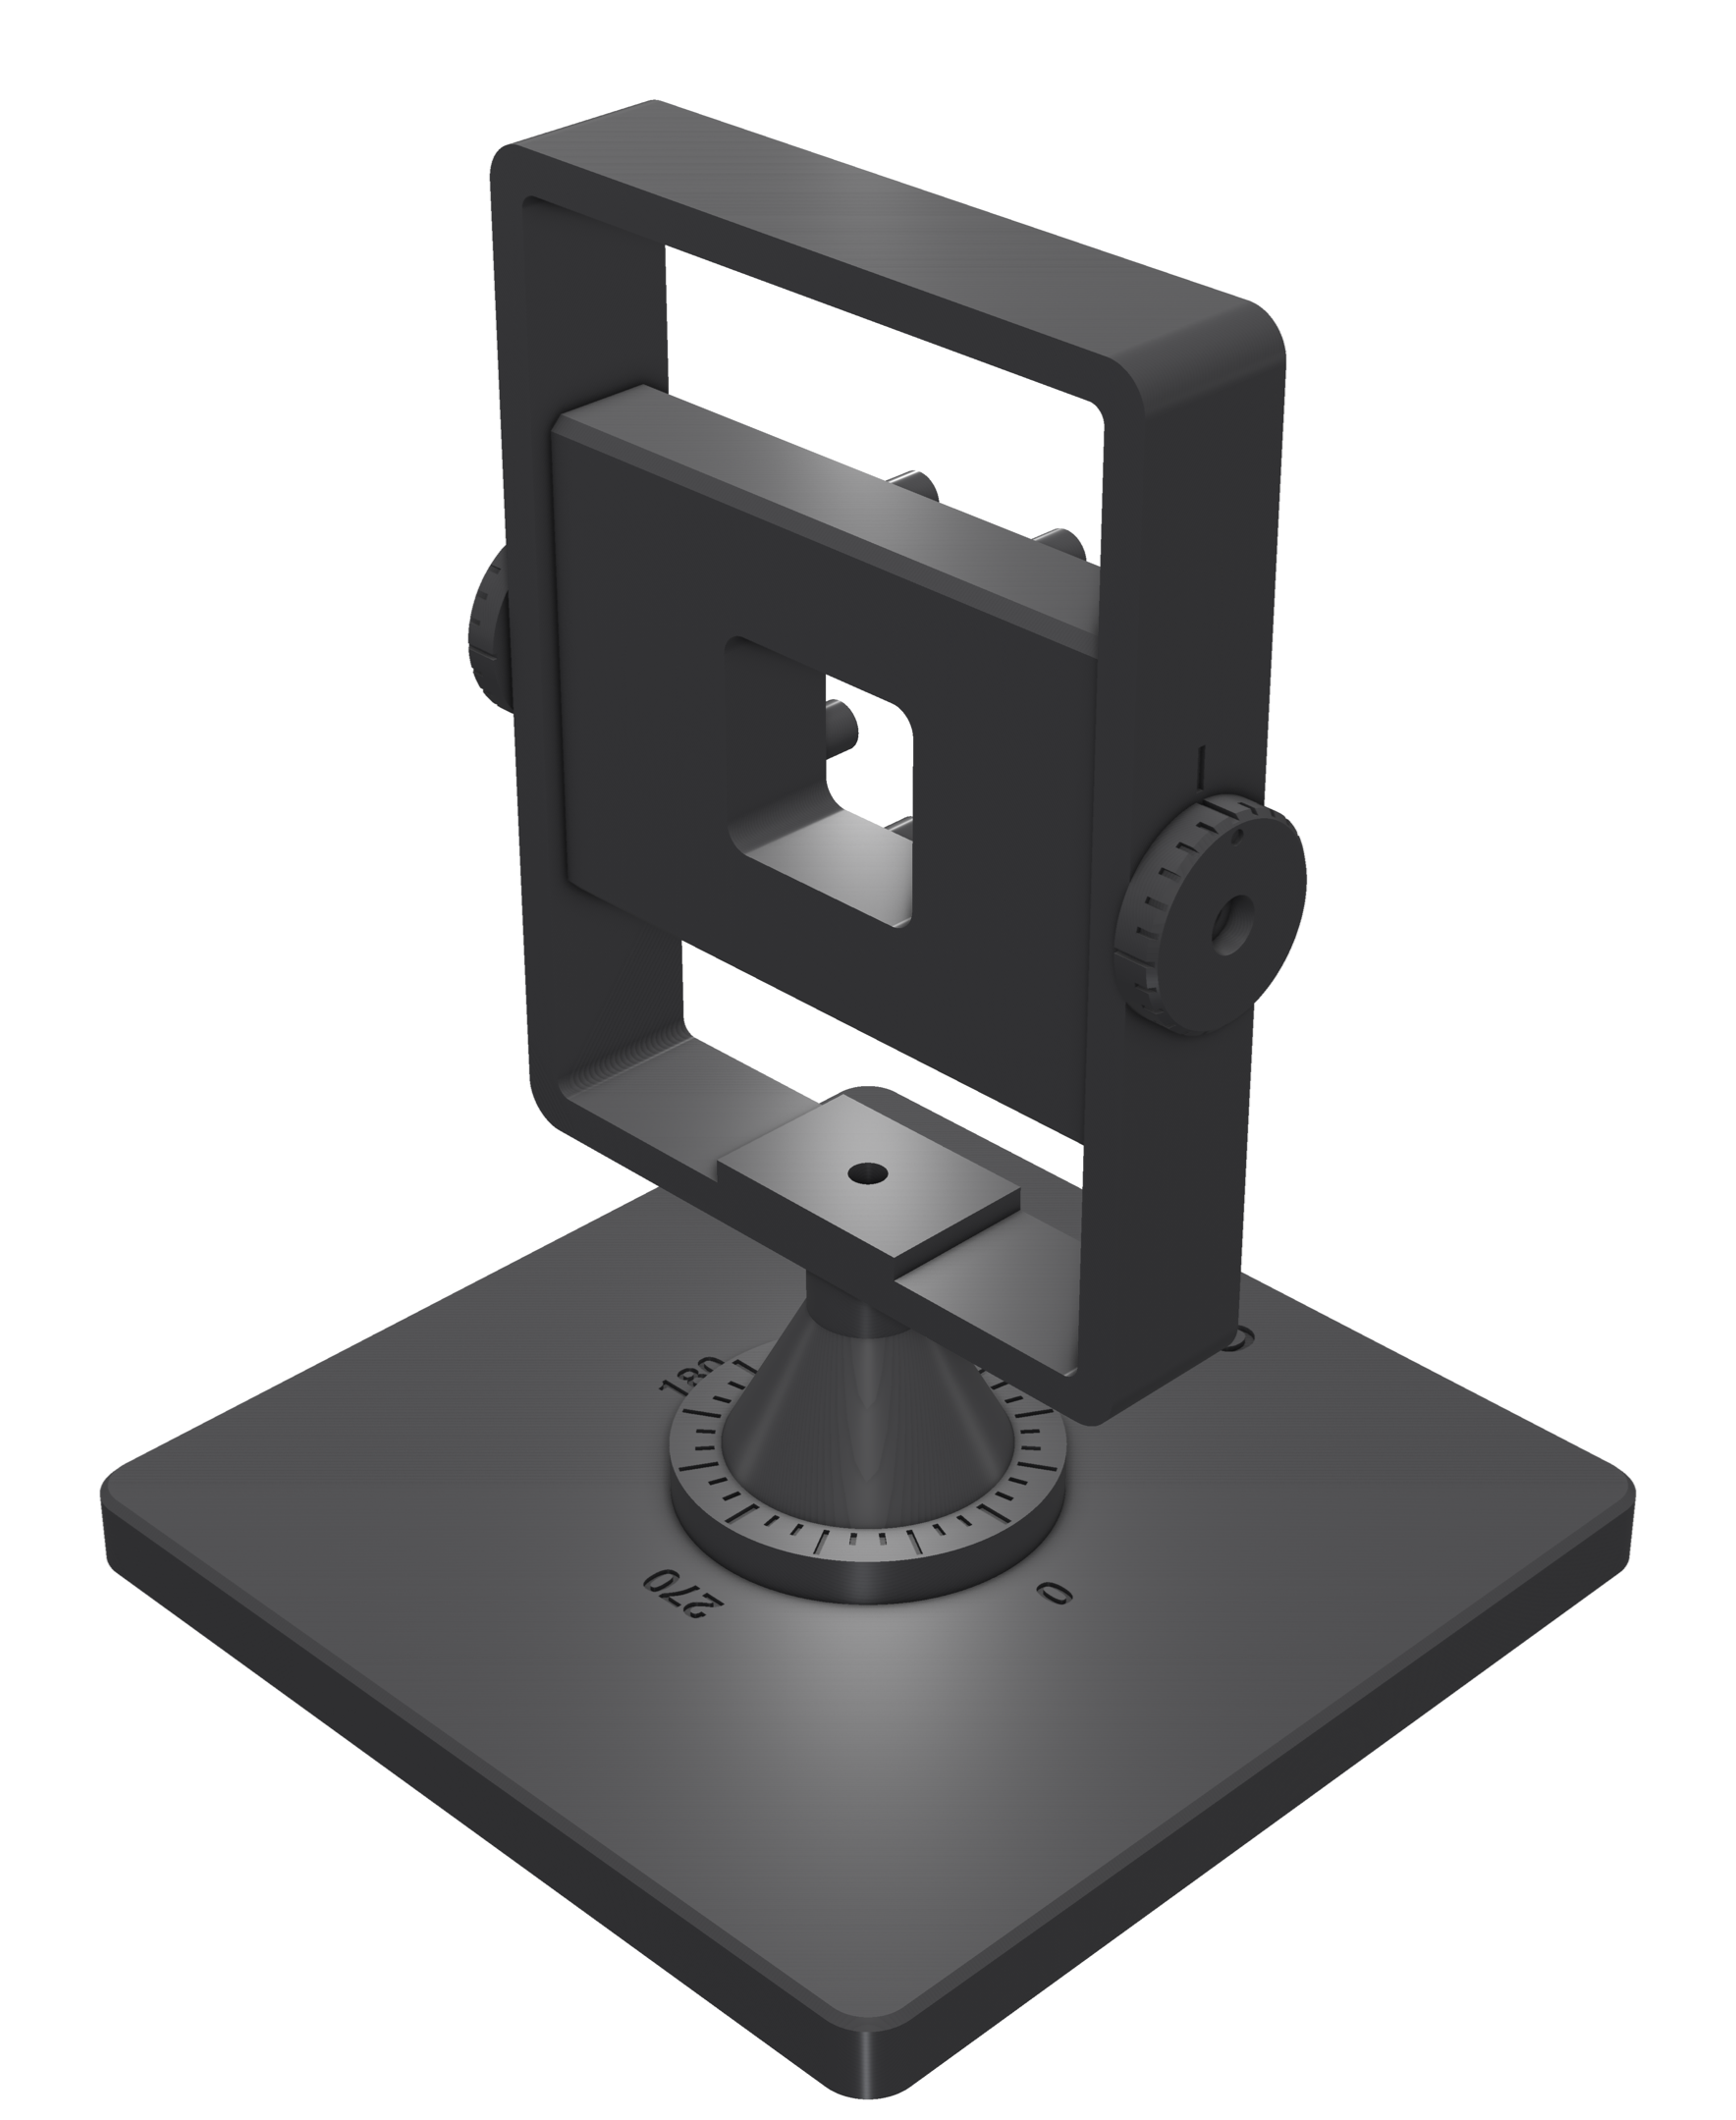
\includegraphics[height=3.3cm]{montagem_render_frente.png}\hspace{2pt}
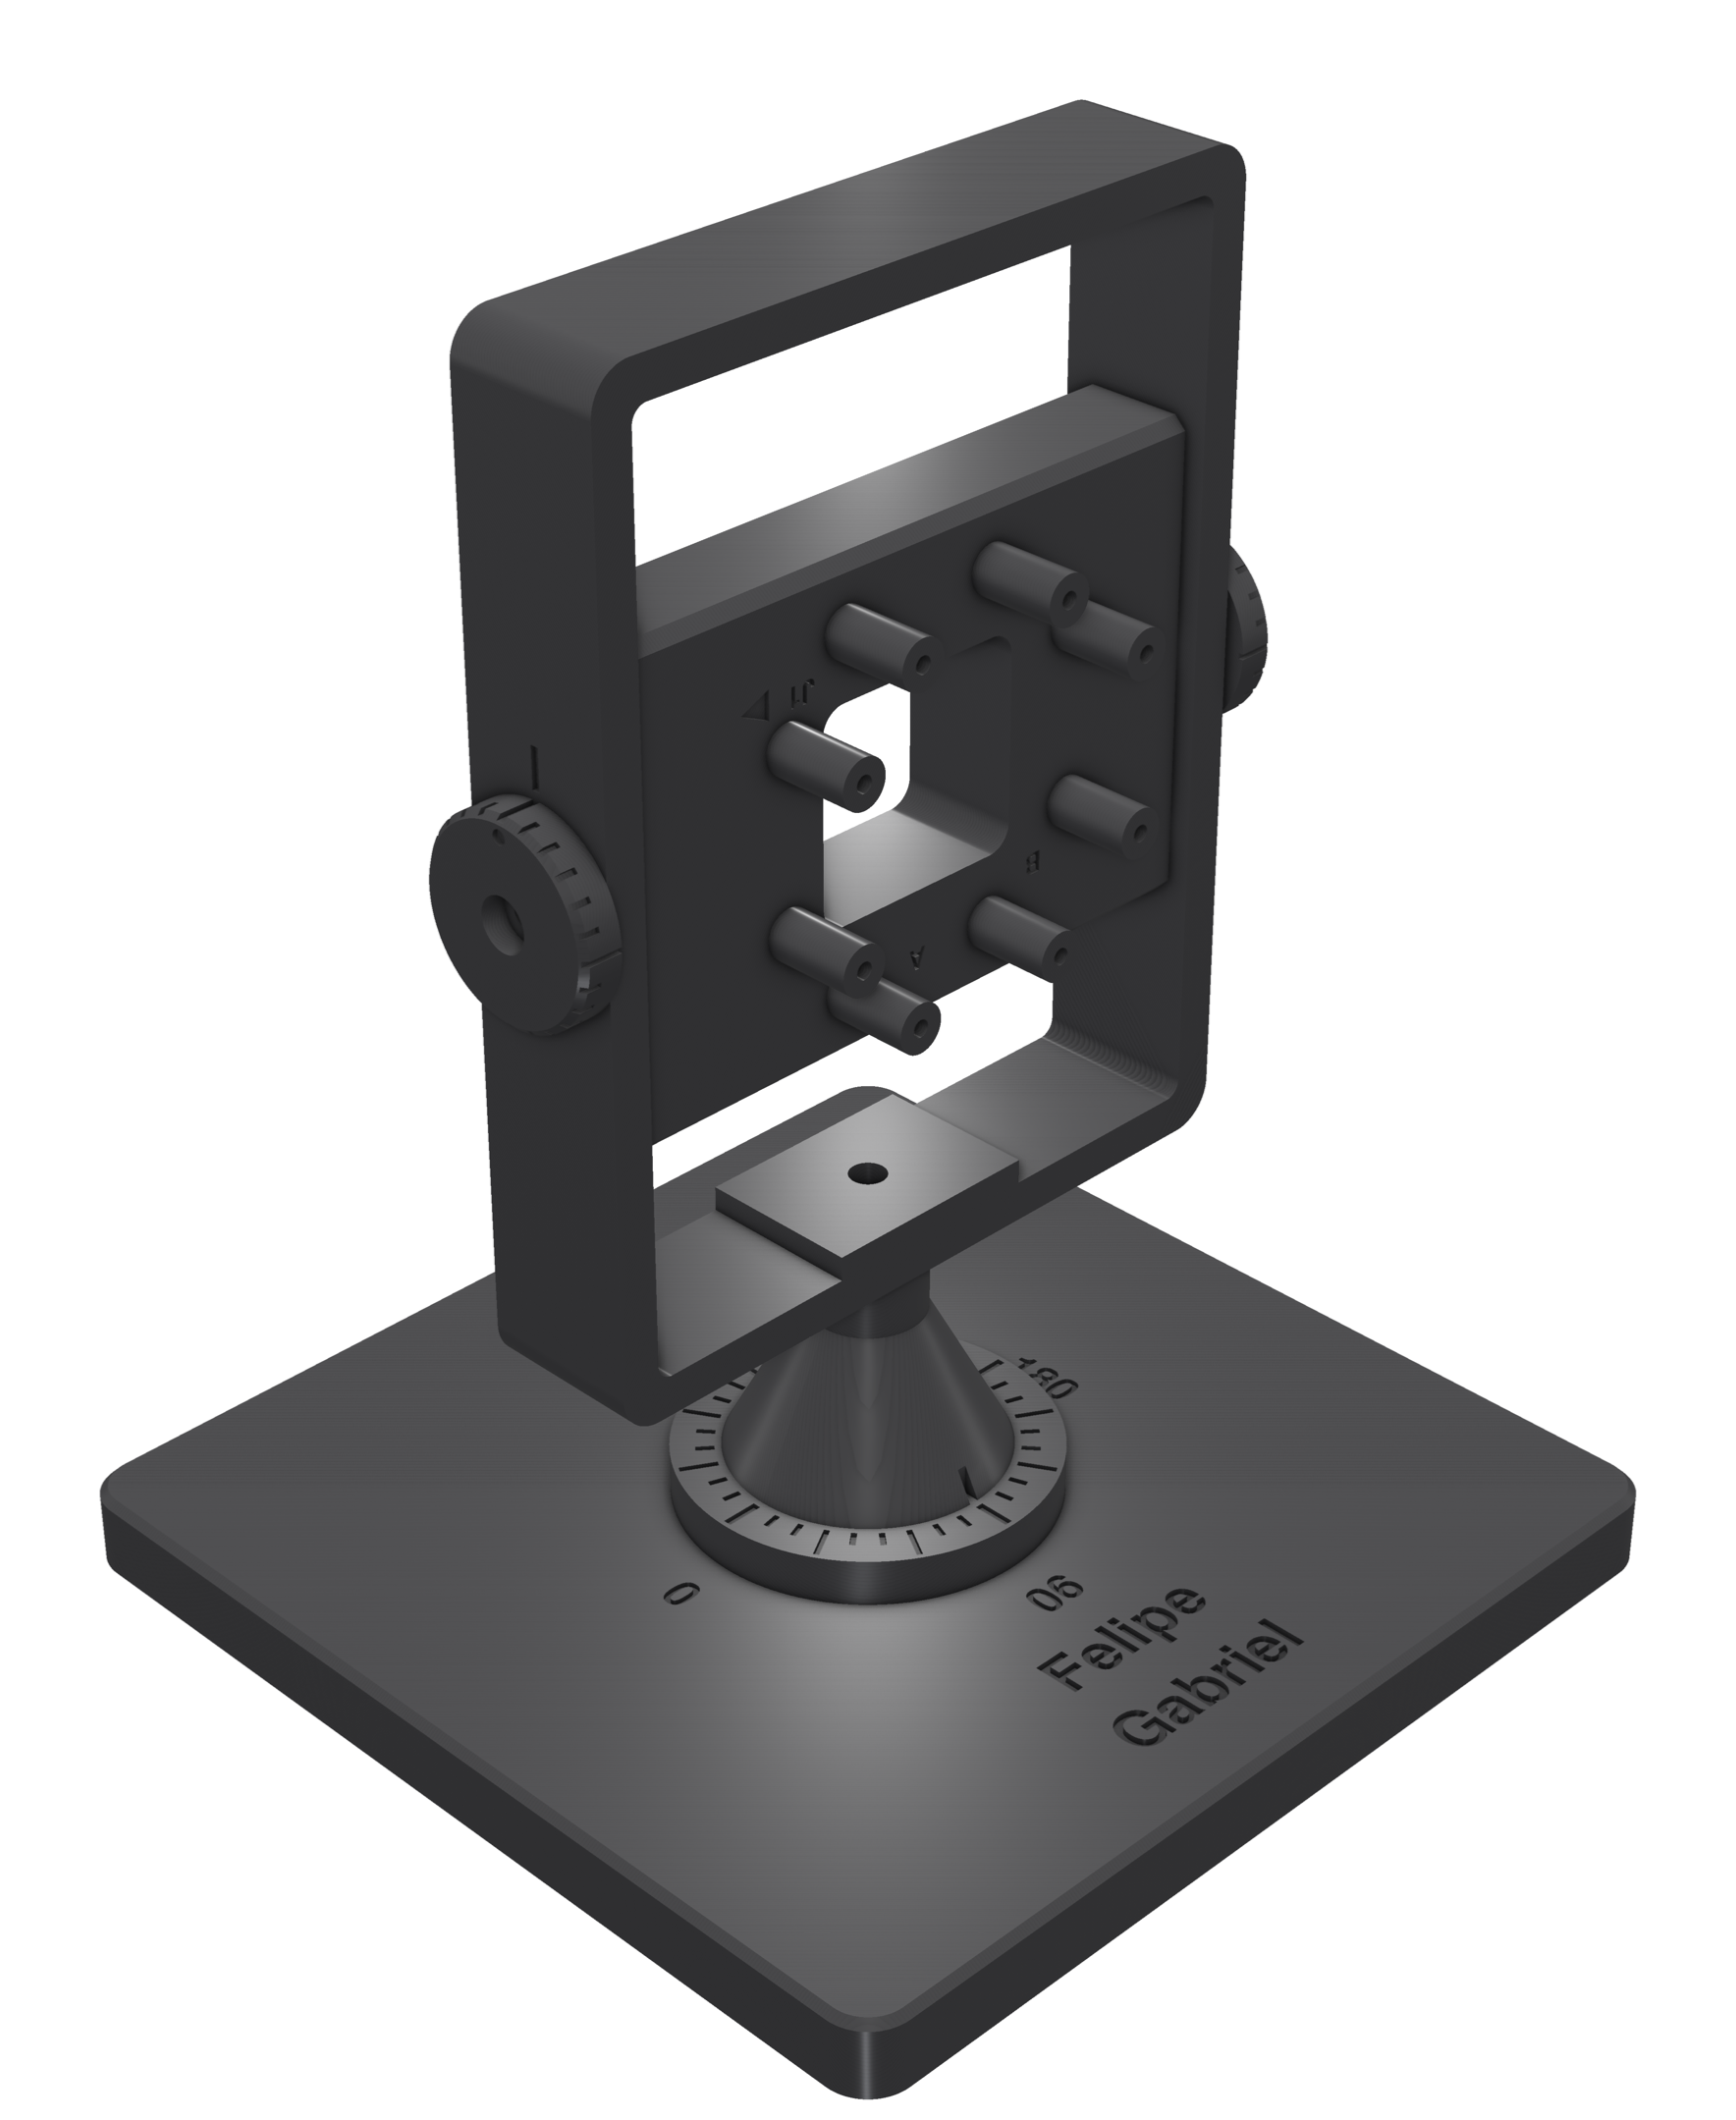
\includegraphics[height=3.3cm]{montagem_render_verso.png}\\[1pt]
\scriptsize Modelo 3D\\[3pt]
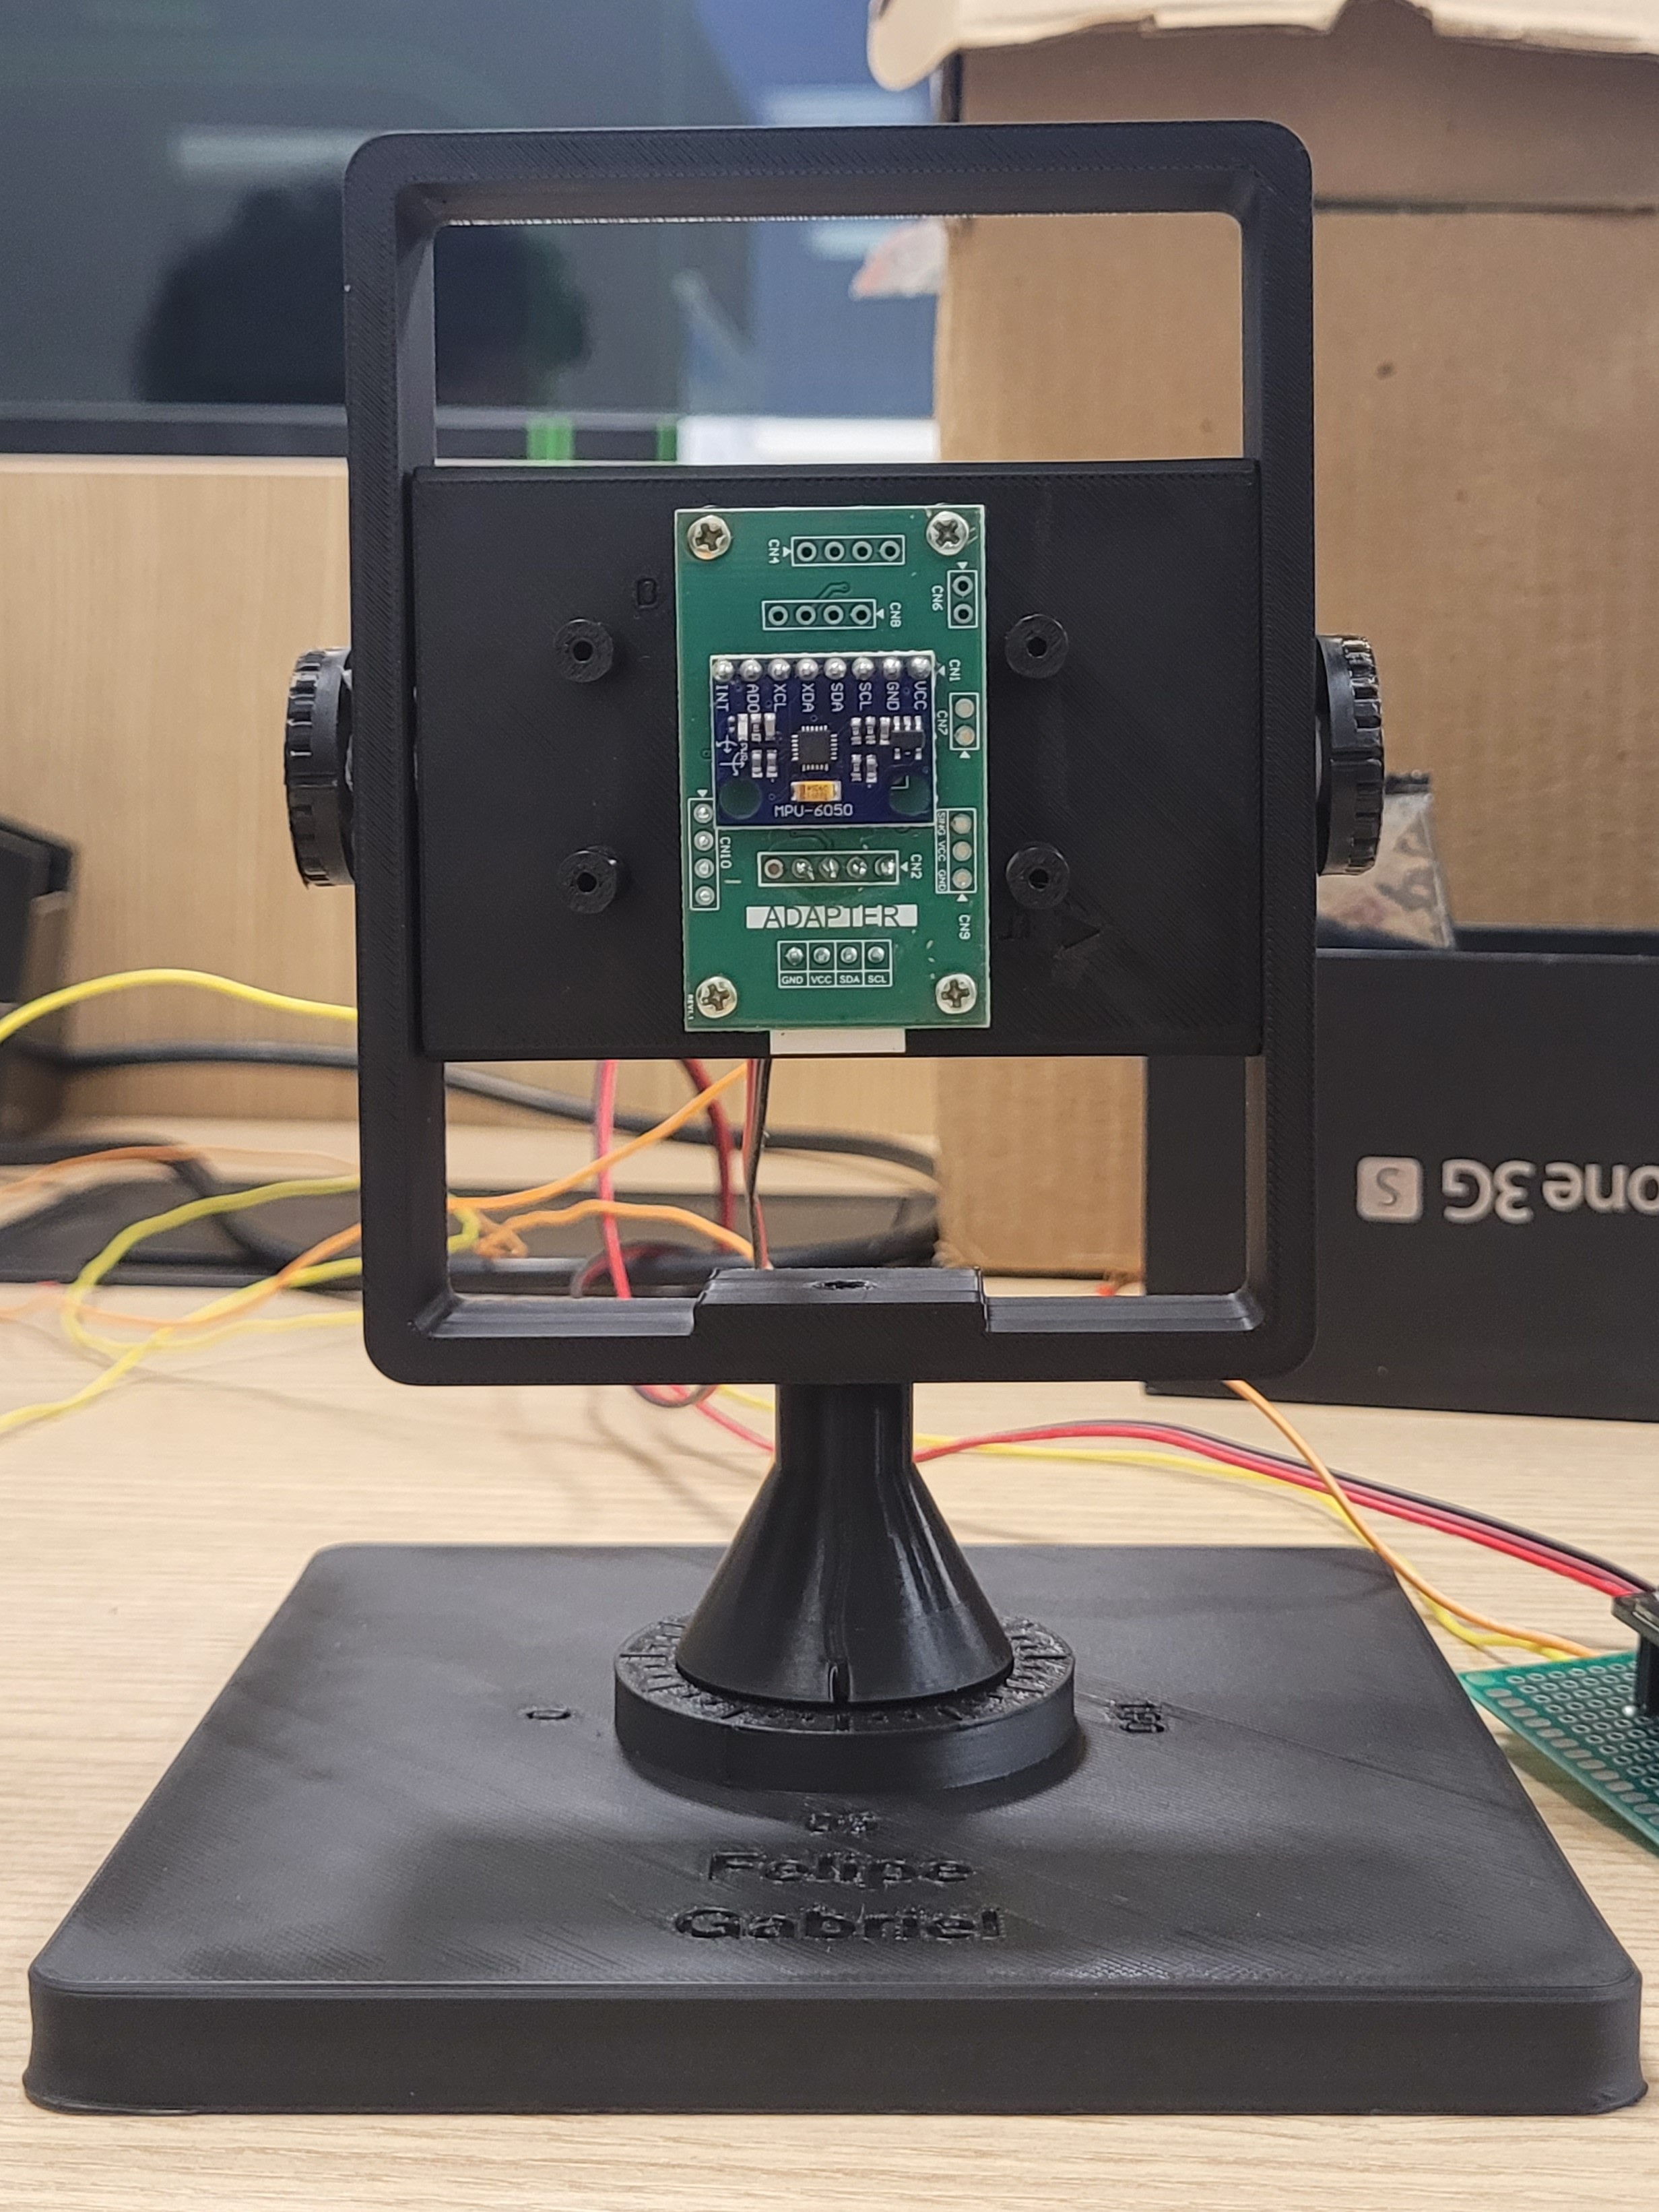
\includegraphics[height=3.0cm]{base_frontal.jpg}\hspace{2pt}
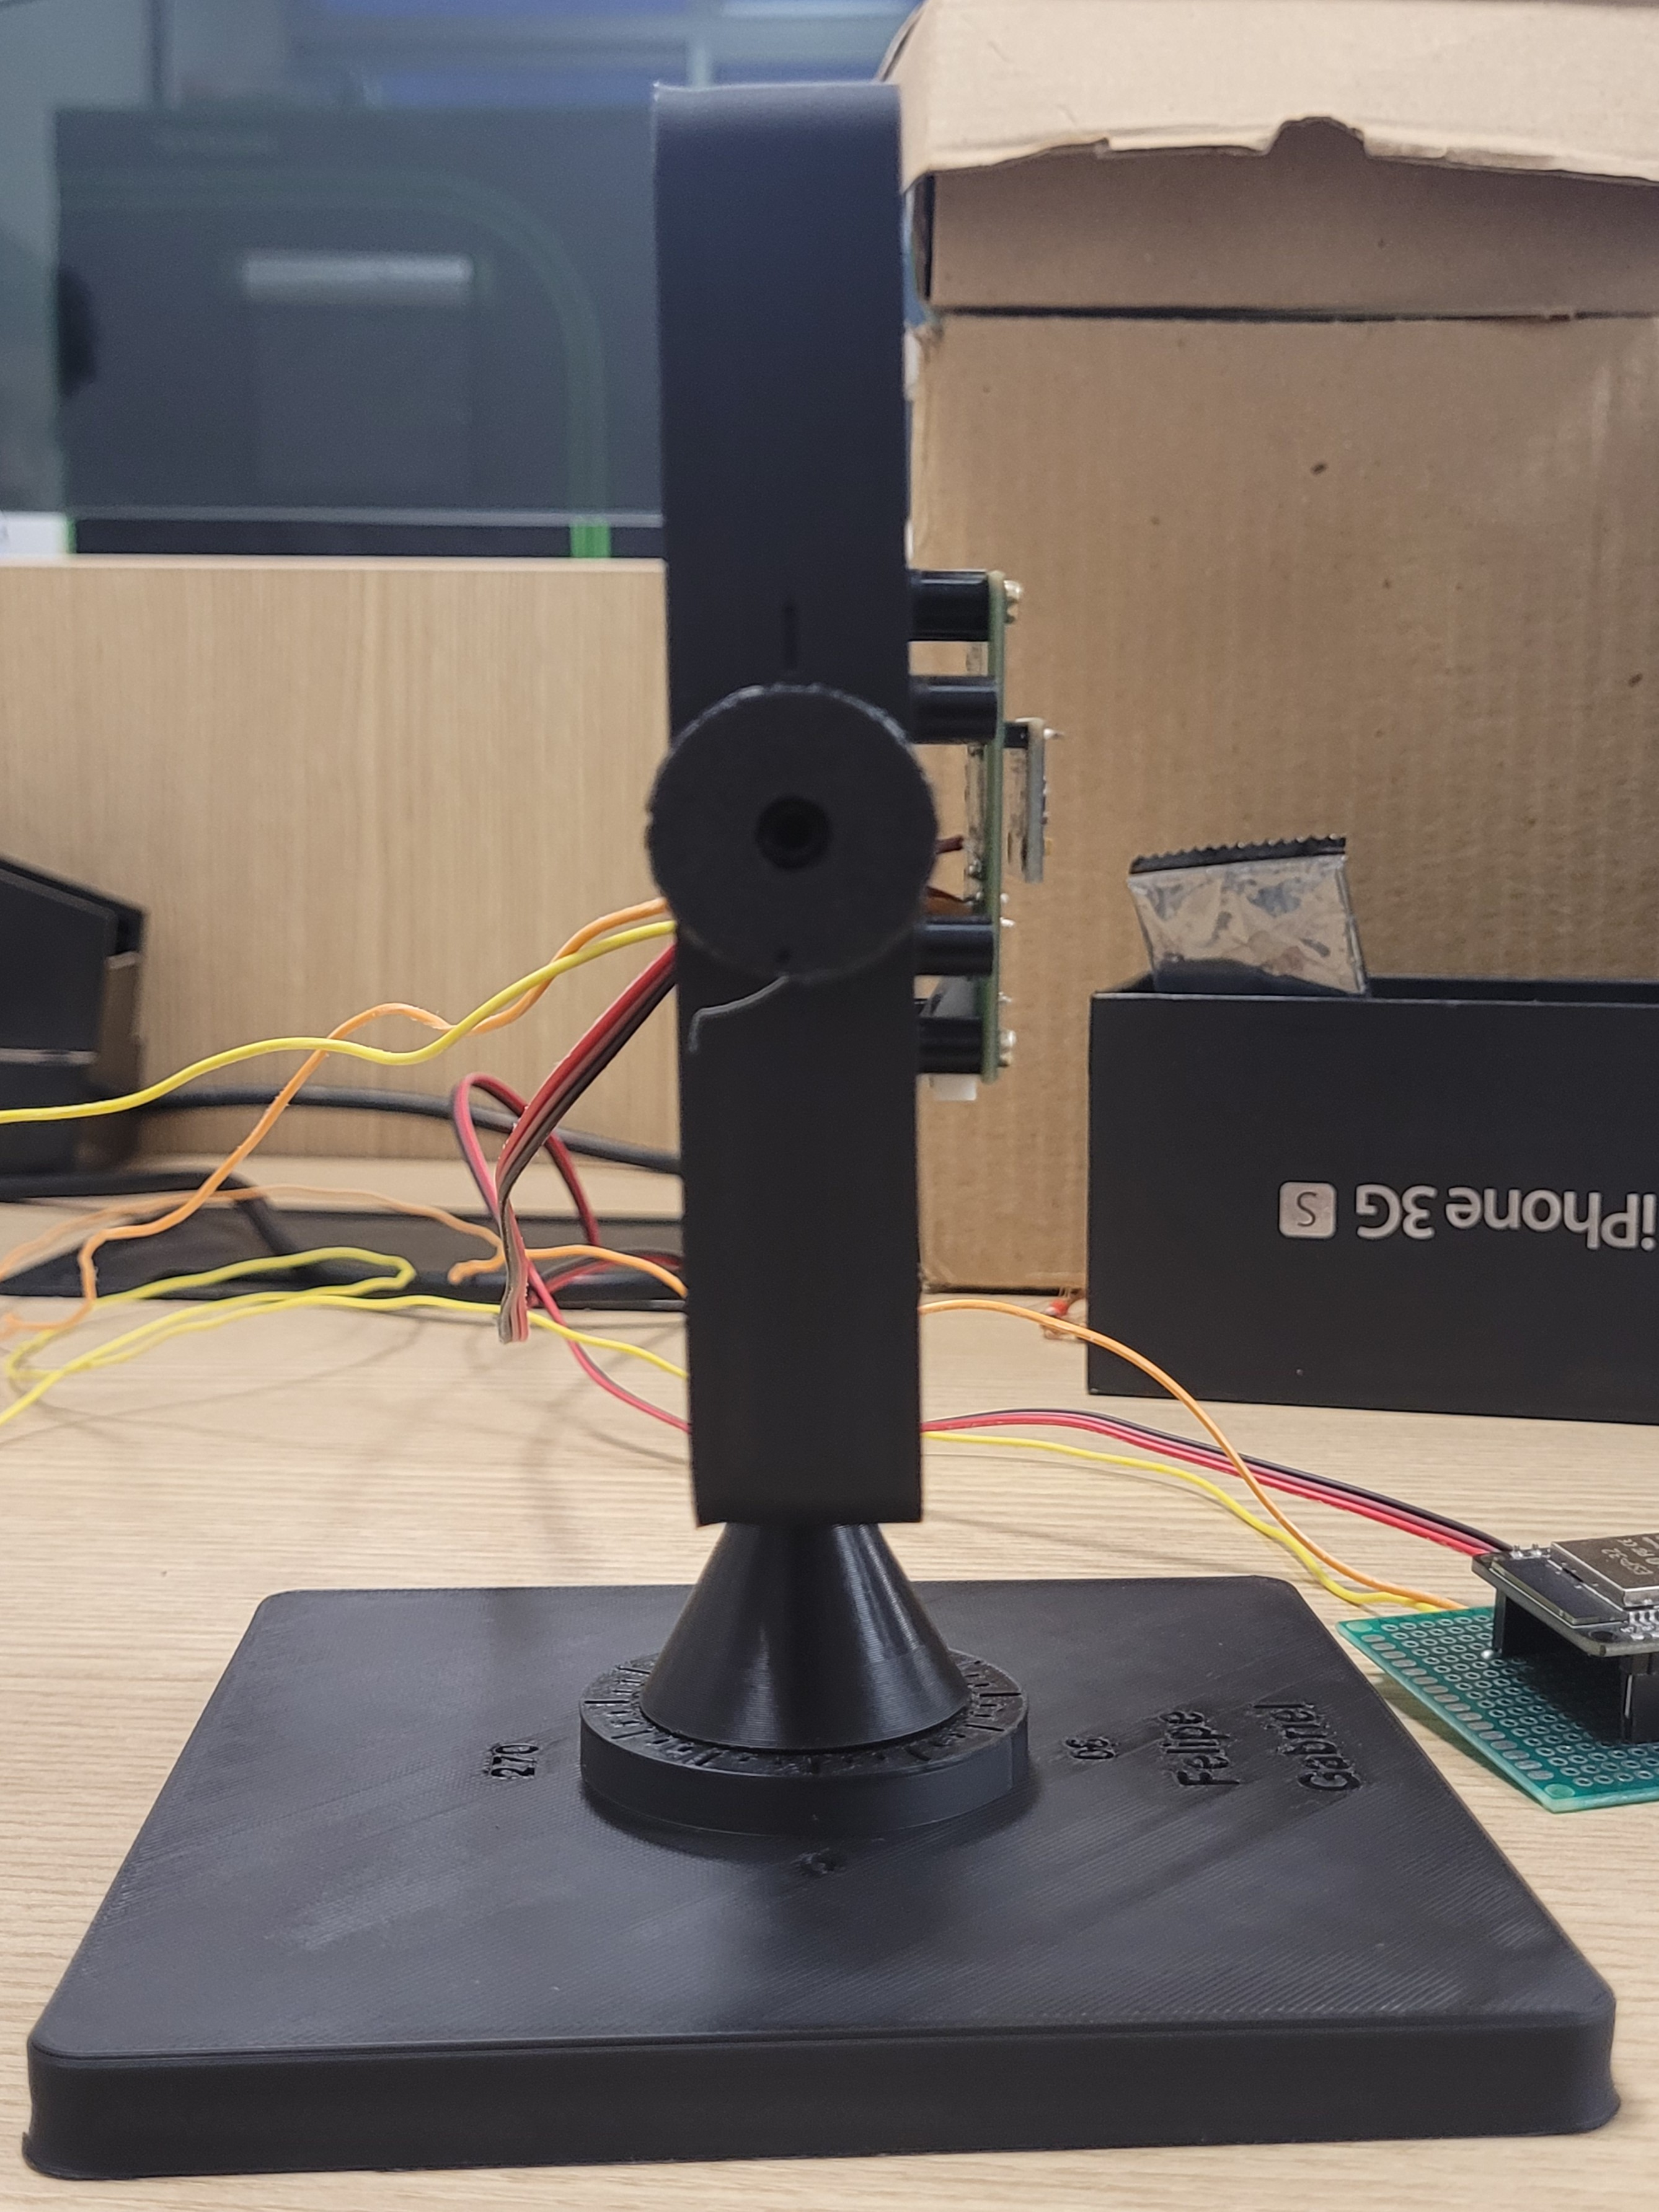
\includegraphics[height=3.0cm]{base_lateral.jpg}\\[1pt]
\scriptsize Base montada
\end{column}
\end{columns}
\end{frame}

% ---------------------------------------------------------------------
\begin{frame}{Calibração estática}
\begin{columns}[T]
\begin{column}{0.44\textwidth}
\small
\textbf{Modelo de cada eixo} (roteiro)
\[
A_{\text{saída}} = \text{Ganho}\times A_{\text{ref}} + A_{\text{offset}}
\]
\textbf{Como foi feito}
\begin{itemize}
\item 6 posições: cada eixo para cima ($+1$\,g) e para baixo ($-1$\,g)
\item Superfície nivelada com nível de bolha
\item 200 leituras por posição, faixa de $\pm2$\,g
\end{itemize}
\end{column}
\begin{column}{0.54\textwidth}
\small
\textbf{Sistema de cada eixo}
\[
\begin{aligned}
\bar{A}_{+1g} &= \text{Ganho}\cdot(+1) + \text{Offset}\\
\bar{A}_{-1g} &= \text{Ganho}\cdot(-1) + \text{Offset}
\end{aligned}
\]
\[
\text{Ganho} = \frac{\bar{A}_{+1g}-\bar{A}_{-1g}}{2},
\quad
\text{Offset} = \frac{\bar{A}_{+1g}+\bar{A}_{-1g}}{2}
\]
\textbf{Correção no firmware}
\[
A_{\text{corrigida}} = \frac{A_{\text{saída}}-\text{Offset}}{\text{Ganho}}
\]
\end{column}
\end{columns}
\end{frame}

% ---------------------------------------------------------------------
\begin{frame}{Resultado da calibração}
\begin{center}
\begin{tabular}{ccccc}
\toprule
Eixo & $\bar{A}_{+1g}$ (g) & $\bar{A}_{-1g}$ (g) & Ganho & Offset (g) \\
\midrule
X & 0,9960 & $-1{,}0015$ & 0,9988 & $-0{,}0028$ \\
Y & 1,0012 & $-0{,}9997$ & 1,0004 & 0,0007 \\
Z & 1,0497 & $-0{,}9810$ & 1,0153 & 0,0344 \\
\bottomrule
\end{tabular}
\end{center}
\vspace{6pt}
\begin{itemize}
\item Ganhos perto de 1 nos três eixos
\item Offset de X e Y abaixo de 3\,mg
\item Offset de Z de 34,4\,mg, dentro do típico do datasheet ($\pm80$\,mg)
\end{itemize}
\vspace{2pt}
\centering\scriptsize Código: \texttt{calibrar.py}
\end{frame}

% ---------------------------------------------------------------------
\begin{frame}{Cálculo do ângulo}
\begin{columns}[T]
\begin{column}{0.5\textwidth}
\small
\begin{itemize}
\item Eixo X do sensor alinhado com o eixo de giro
\item A gravidade fica no plano Y--Z
\item Em $0^\circ$, Y aponta para cima ($c_y = 1$\,g)
\end{itemize}
\[
c_y = \cos\theta,\quad c_z = \sin\theta
\]
\[
\theta = \operatorname{atan2}(c_z,\, c_y)
\]
\begin{itemize}
\item atan2 usa o sinal dos dois eixos e não divide por zero em $90^\circ$
\item Abaixo de $-90^\circ$ soma $360^\circ$: a faixa de 0 a $180^\circ$ fica contínua
\end{itemize}
\end{column}
\begin{column}{0.47\textwidth}
\centering
\begin{tikzpicture}[scale=1.05, >=stealth]
\draw[->, thick] (-0.3,0) -- (3.0,0) node[right] {$Z$};
\draw[->, thick] (0,-0.3) -- (0,3.0) node[above] {$Y$};
\draw[thick] (0,0) circle (0.12);
\fill (0,0) circle (0.035);
\node[below left, font=\scriptsize] at (0,-0.05) {$X$ (eixo de giro)};
\draw[->, very thick, red!70!black] (0,0) -- ({2.5*sin(35)},{2.5*cos(35)}) node[above right, font=\small] {1\,g};
\draw[dashed, gray] ({2.5*sin(35)},{2.5*cos(35)}) -- ({2.5*sin(35)},0);
\draw[dashed, gray] ({2.5*sin(35)},{2.5*cos(35)}) -- (0,{2.5*cos(35)});
\node[below, font=\scriptsize, blue!60!black] at ({2.5*sin(35)},0) {$c_z$};
\node[left, font=\scriptsize, blue!60!black] at (0,{2.5*cos(35)}) {$c_y$};
\draw[->, green!50!black, thick] (0,1.0) arc (90:55:1.0);
\node[green!50!black, font=\small] at (0.3,1.25) {$\theta$};
\end{tikzpicture}\\[4pt]
\scriptsize Referência: notas de aplicação AN3461 e AN-1057
\end{column}
\end{columns}
\end{frame}

% ---------------------------------------------------------------------
\begin{frame}{Programa}
\begin{columns}[T]
\begin{column}{0.5\textwidth}
\small
\textbf{ESP32} (\texttt{main.cpp}, a cada 50\,ms)
\begin{enumerate}
\item Lê $a_x$, $a_y$, $a_z$ e divide por 16384\,LSB/g
\item Corrige com ganho e offset
\item Calcula $\theta = \operatorname{atan2}(c_z, c_y)$
\item Manda pela serial: tempo, $a_x$, $a_y$, $a_z$, $\theta$
\end{enumerate}
\end{column}
\begin{column}{0.47\textwidth}
\small
\textbf{Computador} (Python)
\begin{itemize}
\item \texttt{capturar.py}: grava a serial em CSV
\item \texttt{calibrar.py}: 6 arquivos $\to$ ganho e offset
\item \texttt{erro\_angulo.py}: arquivos de cada ângulo $\to$ gráfico de erro
\end{itemize}
\vspace{6pt}
\scriptsize Códigos no repositório:\\
\texttt{github.com/Gabreeles/}\\
\texttt{instrumentacao\_eletronica\_2026\_2}
\end{column}
\end{columns}
\end{frame}

% ---------------------------------------------------------------------
\begin{frame}{Passo a passo dos ensaios}
\begin{columns}[T]
\begin{column}{0.49\textwidth}
\begin{block}{Calibração}
\footnotesize
\begin{enumerate}
\item Fechar o monitor serial
\item Tirar o módulo do berço e pôr na mesa nivelada
\item Capturar 200 leituras sem encostar na placa:\\
{\tiny\texttt{python capturar.py COM3 calibracao/x\_pos.csv 200}}
\item Repetir nas 6 posições: \texttt{x\_pos}, \texttt{x\_neg}, \texttt{y\_pos}, \texttt{y\_neg}, \texttt{z\_pos}, \texttt{z\_neg}
\item Rodar \texttt{python calibrar.py}
\item Copiar os 6 \texttt{\#define} para o \texttt{main.cpp}
\item Gravar de novo (Upload)
\end{enumerate}
\end{block}
\end{column}
\begin{column}{0.49\textwidth}
\begin{block}{Gráfico do erro angular}
\footnotesize
\begin{enumerate}
\item Pôr o módulo no berço, com X no eixo de giro
\item Conferir no monitor: perto de 0 em $0^\circ$ e de 90 em $90^\circ$
\item Fechar o monitor serial
\item Girar o braço até o ângulo, sempre subindo, e travar
\item Capturar 100 leituras:\\
{\tiny\texttt{python capturar.py COM3 angulos/ang\_0.csv 100}}
\item Repetir 4 e 5 de $15^\circ$ em $15^\circ$ até $180^\circ$ (13 arquivos)
\item Rodar \texttt{python erro\_angulo.py}
\end{enumerate}
\end{block}
\end{column}
\end{columns}
\end{frame}

% ---------------------------------------------------------------------
\begin{frame}{Erro do ângulo}
\slidegrafico{%
\begin{itemize}
\item 13 ângulos, de $0^\circ$ a $180^\circ$ de $15^\circ$ em $15^\circ$
\item 100 leituras em cada ângulo
\item Erro = referência $-$ medido
\end{itemize}
\vspace{4pt}
\scriptsize
\begin{tabular}{@{}lcc@{}}
\toprule
 & com calib. & sem calib. \\
\midrule
Maior erro & $-1{,}23^\circ$ & $-2{,}99^\circ$ \\
RMSE & $0{,}65^\circ$ & $1{,}56^\circ$ \\
Desvio padrão & $0{,}56^\circ$ & $1{,}58^\circ$ \\
Erro médio & $-0{,}23^\circ$ & $-0{,}20^\circ$ \\
\bottomrule
\end{tabular}
}{grafico_erro.png}{erro_angulo.py}
\end{frame}

% ---------------------------------------------------------------------
\begin{frame}{Conclusões}
\begin{itemize}
\item A calibração reduziu o RMSE de $1{,}56^\circ$ para $0{,}65^\circ$ e o maior erro de $2{,}99^\circ$ para $1{,}23^\circ$
\item O erro médio quase não muda porque os erros sem calibração têm sinais diferentes e se cancelam
\item O transferidor tem resolução de $1^\circ$, da mesma ordem do erro medido
\item Vale só para o braço parado: em movimento o sensor também mede a aceleração do movimento
\end{itemize}
\vspace{6pt}
\textbf{Melhorias}
\begin{itemize}
\item Calibrar com o sensor já montado no mecanismo e em mais posições
\item Usar uma referência angular mais exata
\end{itemize}
\end{frame}

% ---------------------------------------------------------------------
\begin{frame}{Demonstração}
\begin{center}
\Large Girando o braço e lendo o ângulo na serial\\[12pt]
\normalsize\texttt{pio device monitor}\\[6pt]
\small A última coluna é o ângulo em graus
\end{center}
\end{frame}

% ---------------------------------------------------------------------
% Sempre o último slide (backup para perguntas)
\begin{frame}{Consulta}
\begin{columns}[T]
\begin{column}{0.48\textwidth}
\begin{block}{Sensor e firmware}
\scriptsize
Faixa $\pm2$\,g: 16384\,LSB/g (0,061\,mg por contagem)\\
Uma leitura a cada 52\,ms (cerca de 19 por segundo)\\
Offset típico do datasheet: $\pm50$\,mg (X, Y), $\pm80$\,mg (Z)
\end{block}
\begin{block}{Fórmulas}
\scriptsize
Ganho $= (\bar{A}_{+1g}-\bar{A}_{-1g})/2$ \quad Offset $= (\bar{A}_{+1g}+\bar{A}_{-1g})/2$\\
$A_{\text{corrigida}} = (A - \text{Offset})/\text{Ganho}$\\
$\theta = \operatorname{atan2}(c_z, c_y)$
\end{block}
\end{column}
\begin{column}{0.48\textwidth}
\begin{block}{Onde estão as coisas}
\scriptsize
\texttt{Entrega\_2/medindo\_angulo/src/main.cpp} -- firmware\\
\texttt{calibracao/} -- 6 posições, 200 leituras\\
\texttt{angulos/} -- 13 ângulos, 100 leituras
\end{block}
\begin{block}{Referências}
\scriptsize
M. Pedley, AN3461 (Freescale) -- inclinação com atan2\\
C. J. Fisher, AN-1057 (Analog Devices) -- um, dois e três eixos\\
InvenSense, datasheet do MPU 6050
\end{block}
\end{column}
\end{columns}
\end{frame}

\end{document}
